\section{Faltung bei ungleicher Spaltbreite}
\subsection* {Theoretischer Hintergrund}
In den Fragen zur Vorbereitung haben wir uns mit der Thematik der Faltung zweier Rechteckfunktionen, besch\"aftigt. Vor allem im Bezug zu unterschiedlichen Ein- und Austrittspaltbreiten haben wir die 
Ergebnisse interpretiert. So haben wir herausgefunden, dass es bei einer Faltung zu einer nach obenhin schmaler werdenden Trapezfunktion f\"uhrt, welche oben ein Plateau in der Mitte besitzt. \\
Sind beide Rechteckfunktionen gleich gro\ss{}, so erh\"alt man eine Dreiecksfunktion mit optimaler Intensit\"at. Die Rechteckfunktionen entsprechen den (Anfangs- bzw. End-)Spaltbreiten. Wenn diese 
unterschiedlich sind, so ist das zu messende Signal kleiner und schw\"acher als bei gleichen Spaltbreiten. Diesen Theoretischen Hintergrund kann man durch unsere Messungen best\"atigen. 

\subsection* {Interpretation} 
Wir betrachten im Folgenden diese Einstellungen bei unseren Messungen:\\\\
1. Eingangsspalt: 1,0mm \tab Ausgangsspalt: 0,5mm\\
2. Eingangsspalt: 0,5mm \tab Ausgangsspalt: 1,5mm\\
3. Eingangsspalt: 0,5mm \tab Ausgangsspalt: 1,0mm\\
4. Eingangsspalt: 0,5mm \tab Ausgangsspalt: 0,1mm\\
 \\
\begin{figure}[h]
    \centering
    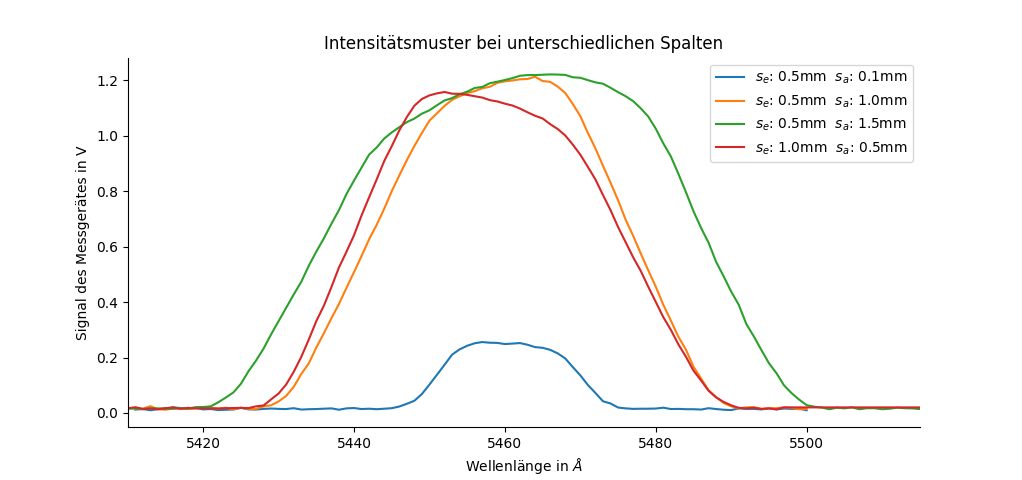
\includegraphics[width = \linewidth]{A5FaltungSpalte.png}
    \caption{Intensitätsmsuter bei unterschiedlichen Ein- und Ausgangsspaltbreiten}
\end{figure}
Bei den Graphen wurde die Intensit\"at gegen die Wellenl\"ange aufgetragen. \\
Im Vergleich zu den vorherig gemessenen Messungen erkennt man, dass es ein deutlich ersichtliches Plateau gibt.
Zus\"atzlich zu beachten ist die geringe Intensit\"at von ca. 1,2 Volt bei den Messungen 1. bis 3. und sogar nur 0,25 Volt bei Messung 4. Der Grund daf\"ur ist die oben angef\"uhrte Faltung von 
Rechteckfunktionen. Die geringe Intensit\"at bei der letzzten Messung ist darauf zur\"uckzuf\"uhren, dass die Spaltbreiten sehr niedrig sind und nah beieinander liegen. Man kann auch erkennen, dass das 
Plateau immer deutlicher zu sehen ist, je h\"oher der Ausgangsspalt ist. Zudem kann man auch einen guten Augenmerk auf die Breite der Messergebnisse legen. Hier merkt man, dass bei der ersten Messung die 
Breite 60 Angstr\"om misst, bei der zweiten Messung 75, bei der dritten wieder 60 und bei der letzten nur 30. Der Grund daf\"ur k\"onnte der Abstand zwischen den Spaltbreiten sein, da sowohl die erste, 
als auch die dritte Messung 0,5mm Unterschied haben. Auch ist zu erkennen, dass je gr\"o\ss{}er eben dieser Abstand ist, desto breiter ist der Graph. \\








